% Chapter Template

\chapter{État de l'art} % Main chapter title

\label{Chapter2} % Change X to a consecutive number; for referencing this chapter elsewhere, use \ref{ChapterX}

%----------------------------------------------------------------------------------------
%	SECTION 1
%----------------------------------------------------------------------------------------
Dans ce chapitre, nous allons voir les principaux concepts impliqués dans l’implémentation d’agents autonomes; les systèmes multiagents avec quelques exemples d’implémentation; la recherche en “NDM” ou prise de décisions en milieu naturel et quelques modèles issus de ces recherches. Aussi, l’architecture BDI (belief, desire, intention) servant à l’implémentation d’agents autonomes et qui représentent l’un des modèles les plus proches de la cognition humaine, ainsi que d’autres architectures.
Nous verrons aussi comment est abordée l’intelligence artificielle dans les jeux vidéo et de quelle manière elle a évolué depuis l’apparition du jeu vidéo ainsi que deux exemples de jeux célèbres implémentant des IA d’une grande complexité.



\section{SMA (ou Système Multi-agent)}

En informatique, un système multi-agent (SMA) est un système composé d'un ensemble d'agents (un processus, un robot, un être humain, etc.), situés dans un certain environnement et interagissants selon certaines relations. Un agent est une entité caractérisée par le fait qu'elle est autonome, ou du moins partiellement.
Objet de longue date de recherches en intelligence artificielle distribuée, les systèmes multi-agents forment un type intéressant de modélisation de sociétés, et ont à ce titre des champs d'applications larges, allant des sciences humaines, jusqu’aux services militaires et médicaux \parencite{sma}.


%-----------------------------------
%	SUBSECTION 1
%-----------------------------------
\subsection{Exemple de SMA de jeu vidéo}

Les communautés virtuelles que l’on trouve de plus en plus dans les jeux vidéo sont un parfait exemple afin de mieux comprendre le fonctionnement d’un SMA. Par exemple, un jeu qui simulerait la vie d’une famille, plusieurs dimensions composent alors ce SMA.

~\par
Premièrement, un environnement, ayant comme paramètre sa taille et qui pourrait se caractériser par la maison et son jardin. Deuxièmement, les agents de ce SMA disposent d’une quantité d’objets dits “passifs” avec lesquels ils peuvent interagir; ce sera l’équipement de la maison ou encore la nourriture. Ensuite, les agents eux-mêmes, actifs et autonomes, ils sont en contact avec tout ce qui les entoure, leur environnement, les objets qui les composent ou encore les autres agents; on les identifie comme étant “les membres de la famille”. On intègre ensuite le concept d’organisation, constituée des différentes relations entre les objets et les agents, liens familiaux, notions de propriété (qui possède tel ou tel objet). Pour finir, on ajoute des opérateurs qui permettent aux agents d’agir sur leur environnement ou sur les autres agents (le fils peut manger un yaourt, promener son chien ou parler à sa sœur) et de capteurs qui permettent aux agents de connaître les changements d'états de leur environnement et des autres agents (le yaourt est tombé par terre, papa m'a demandé de sortir le chien). Voici donc ce que l'on peut appeler un SMA \parencite{sma}.


\subsection{Exemple de SMA en opération “SWARMM” (Smart Whole Air Mission Model)} \label{ssec:swarm}

Le  programme “SWARMM” \parencite{jones1999automated} a été développé par la division des opérations aériennes de l’organisation australienne de défense, de science et technologies; il a  pour objectif de simuler les opérations des avions de combat pour la flotte aérienne australienne la “Royal Australian Air Force”.

~\par
Chaque pilote est un agent programmé avec dMARS \parencite{dmars1997formal}, un environnement de programmation basé sur le modèle BDI (Belief-desire-intention ou Croyance-désir-intention) et implémenté en FORTRAN et en C. Chacun d'entre eux reçoit des données des modèles physiques équivalentes à celles qu'un pilote reçoit de sa vision et de ses instruments et effectue ce qui suit:

~\par
\begin{itemize}
\item cycle de prise de conscience de la situation lorsque les données sont plus complexes (descripteurs symboliques);
\item  évaluation de la situation, la situation est basée sur les résultats précédents de l'étape précédente;
\item sélection tactique, sélectionnée en fonction de l'ensemble actuel d'objectifs qui a été reconnu lors des étapes précédentes;
\item procédures d'opération: choisies pour mettre en œuvre une tactique.
\end{itemize}

~\par
Plus d'une décennie de contacts étroits, d'entretiens avec des combattants, de briefings de missions et d'implication dans des exercices d'entraînement a été nécessaire afin d’arriver à établir ce cycle. Il s’est avéré être d’une très grande valeur car il permet une intégration simple des procédures standards et de manière très documentée. Il permet aussi aux combattants de décrire facilement leurs connaissances en se basant sur les différentes étapes du cycle. Pour finir, il assure un échange simple compris entre les deux partis, pilotes et programmeurs. Les programmeurs peuvent ainsi décrire leurs résultats et débattre avec les pilotes en utilisant des termes similaires. Ce programme est principalement  basé sur le travail d’équipe et s’est avéré être extrêmement utile pour tester de nouveaux équipements et tactiques.

~\par
L’un des principaux buts du projet était l’introduction d’un pilote (agent humain) dans la boucle de simulation en tant que coéquipier ou adversaire. Il a donc été prouvé que même si pour un observateur extérieur, ce programme ressemble à un vrai pilote, il n’était pas crédible aux yeux des vrais pilotes, et cela aux vues de son comportement extrêmement rationnel et peu naturel \parencite{norling2000enhancing}.


\section{Naturalistic Decision Making (NDM)} \label{ndm}

\begin{quotation}
“L’étude de la NDM  pose la question de comment des individus expérimentés, travaillant individuellement ou en groupes, dans un environnement dynamique, rapide et incertain, identifient et évaluent leurs situations, prennent des décisions et effectuent des actions qui ont des conséquences signifiantes sur eux ainsi que sur l'organisation dans laquelle ils opèrent.” \parencite{zsambok2014naturalistic} \end{quotation} 



Ce terme est apparu en 1989 lors d’ateliers de chercheurs qui avaient pour but d’étudier 
“les prises de décisions dans des contextes réalistes” (médecine, centrales nucléaires, planification exécutive). Leurs études ont montrés que les théories classiques sur les prises de décisions n’étaient tout simplement pas applicables dans le monde réel. Ils ont aussi prouvé que même lorsque les agents étaient entraînés à faire des choix rationnels, ces derniers ne le faisaient que rarement.

~\par
Il en a ainsi émergé une meilleure compréhension sur la manière dont nous procédons pour prendre des décisions dans des situations complexes. Dans certains cas, nous procédons effectivement de manière rationnelle, où, une multitude d’options sont générées et la “meilleure” est sélectionnée, mais il existe d’autres stratégies qui sont plus communément utilisées.

~\par
La recherche dans ce domaine est principalement destinée à la conception d’aides à la décision, mais ces résultats peuvent également être utilisés pour développer de meilleurs modèles cognitifs pour les humains lors des simulations.

~\par
Orasanu et Connolly \parencite{orasanu1993reinvention} énumèrent huit facteurs qui caractérisent les paramètres de prise de décisions en milieu naturel. De nombreuses études de prise de décisions classiques ignorent ou limitent délibérément ces facteurs, ce qui rend la théorie du choix rationnel plus facile à appliquer.

~\par

Ces facteurs sont:
\begin{itemize}
\item problèmes mal structurés;
\item environnements dynamiques incertains;
\item objectifs changeants, mal définis ou concurrents;
\item boucles d'actions / de rétroactions;
\item le stress dû au temps;
\item des enjeux trop élevés;
\item plusieurs joueurs;
\item objectifs organisationnels et normes.
\end{itemize}

~\par
Tous ces facteurs ne sont pas présents dans un contexte dit “naturel”, mais chacun ajoute une complexité au problème.


\subsection{Modèles de NDM}

Plusieurs modèles de prise de décisions en milieu naturel ont été proposés, mais à ce jour,
aucun d’entre eux ne rend compte du spectre complet des décisions pouvant être prises dans un contexte naturel. Lipshitz \parencite{lipshitz1993converging} donne un résumé de neuf modèles qu’il souligne être non contradictoires, mais illustrent les différents types de prise de décision qui peuvent être utilisés.

~\par
Notez que les chercheurs en NDM s'intéressent généralement aux personnes qui sont expérimentées dans leurs domaines. Hubert Dreyfus explique le modèle d’acquisition de compétences en cinq étapes dans \parencite{dreyfus2014intuitive}, avec des niveaux allant de novice (quelqu'un qui débute dans  le domaine, comme un apprenti pilote), à un expert (quelqu'un qui est très habile dans son activité). La plupart des modèles NDM supposent un certain niveau d'expertise dans le domaine, pas nécessairement expert, mais certainement pas novice. L’un des modèles les plus connus est celui de Klein intitulé  “recognition-primed decision making”, modèle (RPD), ou “la prise de décision axée sur la reconnaissance” \parencite{klein2017sources}, illustré à la figure \ref{fig:klein}.

~\par 
Comme le souligne Klein lui-même «Le modèle RPD n'est pas issu de recherches en NDM» (\parencite{klein2017sources}, p.102), mais des études d’experts dans divers domaines montrent qu’une grande partie de leurs décisions sont prises de cette façon (figure \ref{fig:klein}). La chose importante à noter à propos de ce modèle est l'accent qui est mis sur l'évaluation de la situation. Une fois que le décideur a reconnu la situation, il existe quatre sous-produits:

\begin{enumerate}

\item il / elle s'attend à ce que certaines choses se produisent mais pas d'autres;
\item il / elle fait attention à certains signaux pour soutenir le diagnostic;
\item il existe une certaine compréhension des objectifs qu'il est plausible de réaliser;
\item certaines actions sont susceptibles de réussir.
\end{enumerate}

Le décideur choisit ensuite une action, exécute une rapide simulation mentale de
celle-ci, et s'il/elle pense que cela va réussir, la met en œuvre. Une fois que le plan d’action  a été sélectionné et qu’il est entamé, la situation est surveillée pour s’assurer qu’elle se déroule comme prévu, sinon, d’autres actions pourraient être envisagées, mis à part cette éventualité, le décideur n'envisage pas d'autres options. Dans le modèle RPD, un opérateur expérimenté
choisira généralement «automatiquement» un plan d’action une fois que la situation est
reconnue, et que ce plan d’action est susceptible d’être celui qui a donné  auparavant
des résultats positifs dans la même situation.


\begin{figure}[th]
\centering
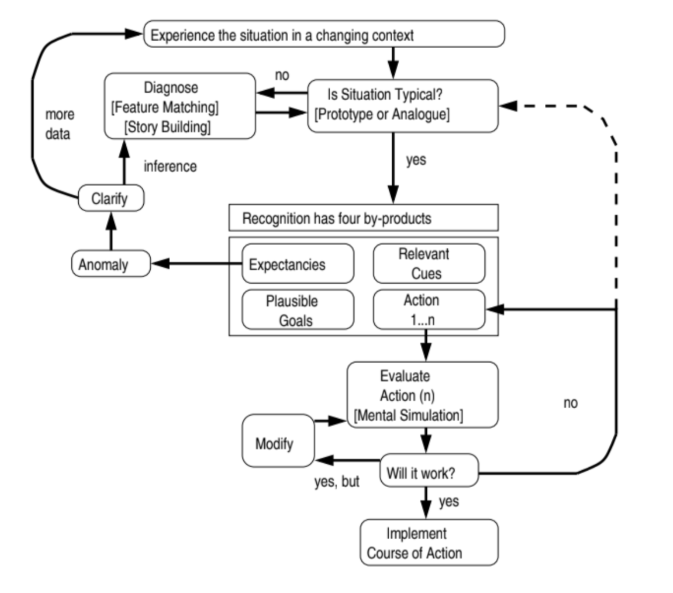
\includegraphics{Figures/klein.PNG}
\decoRule
\caption[ La version intégrée  du modèle de Klein de décision axée sur la reconnaissance] { La version intégrée  du modèle de Klein de décision axée sur la reconnaissance
(Figure 7.1 du livre “Sources of Power” by G. Klein 1998 \parencite{klein2017sources}) }
\label{fig:klein}
\end{figure}


~\par
Le modèle de la figure \ref{fig:klein} exprime l’idée qu’une personne qui acquiert de l’expertise est plus susceptible 
de reconnaître les subtilités entre les situations et de choisir un plan d’action en conséquence.



~\par

\section{Une brève histoire des jeux dans la recherche sur l'IA}

Les jeux ont une longue histoire dans la recherche sur l'IA, remontant au moins à 1949 lorsque Claude Shannon (peu après avoir développé l'entropie d'informations) s'est intéressé à l'écriture d'un programme informatique pour jouer au jeu d'échecs \parencite{unity2}. Dans son article «Programmer un ordinateur pour jouer aux échecs», Shannon écrit:

~\par
“La machine à échecs est un système idéal pour commencer, car: 

~\par
\begin{enumerate}
\item le problème est clairement défini à la fois dans les opérations autorisées (les mouvements) et dans le but ultime (le mat); 
\item il n'est ni si simple jusqu'à être trivial ni trop difficile; 
\item les échecs sont généralement considérés comme nécessitant une «réflexion»; une solution à ce problème nous obligera soit à admettre la possibilité d'une pensée mécanisée, soit à restreindre davantage notre concept de «pensée»; 
\item la structure discrète des échecs s’intègre parfaitement dans la nature numérique des ordinateurs modernes.”

\end{enumerate}

C'était en 1949.

~\par
Depuis lors, il existe un intérêt considérable pour la création de programmes informatiques capables de jouer à des jeux de manière aussi habiles que des joueurs humains, parfois même en battant les meilleurs. Shannon a inspiré le travail fondateur d’Arthur Samuel sur Checkers entre les années 1950 et 1960. Si le programme de Samuel n’a pas pu battre les experts, il a été considéré comme une réalisation majeure, car il s’agissait du premier programme à utiliser efficacement les procédures de recherches heuristiques et les méthodes basées sur l’apprentissage \parencite{unity1}.


~\par
Chinook, un programme de contrôleurs mis au point à l’Université d'Alberta en 1989, a commencé à battre les joueurs humains, et dès 1994, les meilleurs joueurs pouvaient au mieux être à égalité avec la machine. Cette tendance s’est poursuivie avec d’autres jeux de plateau à 2 joueurs tels que le backgammon (avec TD-Gammon de Gerald Tesauro, 1992-2002) et le jeu d'échecs (lorsque Deep Blue d’IBM a battu Garry Kasparov, 1997), et plus récemment avec Go.

~\par
Une avancée scientifique importante de ces dernières années a été celle où, en 2016, AlphaGo de DeepMind a battu le champion du monde Lee Sedol 18 fois 4 à 1, faisant l’objet du documentaire Netflix, AlphaGo \parencite{unity2}. 



\section{BDI ( Belief-Desire-Intention)}

Les agents du modèle BDI sont basés sur les concepts philosophiques d'intentions, de plans et de raisonnements pratiques développés par Bratman \parencite{bratman1987intention}. Ce modèle est basé sur la psychologie populaire, c'est-à-dire la manière dont nous pensons. Le modèle fournit une première approximation de la cognition humaine, mais il reste encore beaucoup à faire pour l’affiner.


\subsection{Belief}

Les croyances d'un agent sont sa vision du monde, qui n'est pas nécessairement la même chose que l'état du monde, car les capteurs peuvent être imparfaits, en effet, les informations fournies peuvent être à la fois incomplètes et bruyantes.

\subsection{Desire}

Plutôt que les désirs d’un agent, nous nous référons à ses objectifs. Ceux-ci donnent l'état du monde dans lequel l'agent souhaite être et doit être cohérent.


\subsection{Intention}

Ses intentions sont les plans qu'il exécute actuellement. Il peut y avoir plus d'un plan en cours, car un agent peut travailler simultanément à plusieurs objectifs (non conflictuels). Une fois qu'un agent a formulé une intention (c.-à-d. il sélectionne un plan), il est en quelque sorte engagé dans ce plan - il continue de l'exécuter (ou du moins a l'intention de l'exécuter) jusqu'à ce que l'objectif soit atteint ou qu’il devienne impossible à atteindre en suivant ce même plan, l'objectif devient alors inutile. 
Un plan est une «recette» pour atteindre un objectif particulier. C'est une séquence d'actions et/ou de sous-objectifs à réaliser. Si une étape de la séquence échoue, le plan lui-même échouera. L'une des caractéristiques d'un système BDI est que, lorsqu'un plan échoue, l'agent réessaye (si possible). Il tentera de trouver un autre moyen d’atteindre l’objectif en tenant compte du fait que le monde (et donc les convictions de l’agent ou son désir) est en train de changer. Un agent stocke ses plans dans une bibliothèque de plans.


\subsection{Agent BDI} \label{bdiA}

L'agent montré à la figure \ref{fig:bdi}, page \pageref{fig:bdi} \parencite{norling2000enhancing} passe par un cycle continu de:

\begin{enumerate}
\item visualiser son environnement;
\item raisonner sur les croyances, les objectifs et les intentions;
\item accomplir une ou plusieurs actions.
\end{enumerate}

Ce cycle est très similaire à celui utilisé dans SWARMM section \ref{ssec:swarm}, qui sépare la deuxième étape en deux étapes: évaluation de la situation suivie de la sélection tactique. En effet, SWARMM est implémenté en utilisant une architecture BDI. Au cours de la phase de raisonnement du cycle, l'agent doit raisonner sur les croyances (si et comment elles devraient changer), les objectifs (les changements de croyances peuvent affecter la faisabilité des objectifs) et les intentions (les changements d'objectifs peuvent amener l'agent à abandonner certaines intentions et / ou d’en créer de nouvelles). L'agent doit également décider quelle action (ou quelles actions) effectuer ensuite, à partir des intentions actuelles.


\begin{figure}[th]
\centering
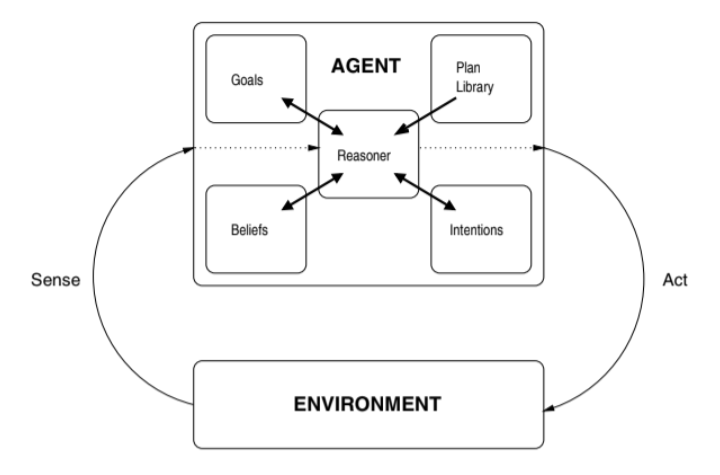
\includegraphics{Figures/bdi.PNG}
\decoRule
\caption[ Structure d’un agent BDI ] { Structure d’un agent BDI }
\label{fig:bdi}
\end{figure}


~\par
Lorsqu'il existe plusieurs plans disponibles pour atteindre un objectif donné, l'agent utilise en théorie un choix rationnel pour sélectionner un plan \parencite{bratman1988plans}. C'est-à-dire que les avantages de tous les plans applicables sont évalués et que le «meilleur» est sélectionné. Cependant la recherche en NDM indique que ce n'est pas ainsi que les agents humains prennent leurs décisions, et c'est sur cela que le travail doit être fait pour  améliorer le modèle BDI .

~\par
Dans les implémentations pratiques d'architectures BDI, telles que JACK \parencite{jack} ou dMARS \parencite{dmars1997formal}, chaque plan est conçu pour gérer un objectif particulier dans un contexte particulier. Dans ces systèmes, le "contexte" est un ensemble de conditions que l'agent doit croire vraies. Cela permet au programmeur de spécifier différentes manières d'atteindre le même objectif dans différentes situations, mais il est également possible d'avoir plusieurs plans applicables dans une situation donnée (lorsque les contextes se chevauchent).







\section{Autres modèles et architectures}

\subsection{CogAff} \label{cogaff}

CogAff est un modèle de traitement de l'information proposé par Sloman \parencite{sloman2005architectural}. Il comprend trois niveaux, à savoir: réactif, délibératif et réflexif (méta-gestion). 
Chaque niveau comprend des mécanismes de perception, des mécanismes de traitement centralisés et des mécanismes d'action. L'architecture possède un mécanisme d'alarme ainsi que des communications d'informations entre toutes les parties de l'architecture. Le mécanisme d'alarme fonctionne de manière centralisée et s'apparente au mécanisme d'interruption.

~\par

H-CogAff est un exemple particulier de CogAff expliquant les phénomènes mentaux humains. Chaque niveau supporte différentes catégories d'émotions. «D'autres subdivisions sont nécessaires pour couvrir toute la variété des émotions humaines, d'autant plus que les émotions peuvent changer de caractère au fil du temps, à mesure qu'elles grandissent» \parencite{sloman2005architectural}.


\subsection{CLARION}

CLARION a une structure similaire aux trois niveaux de traitement de l’information (section \ref{cogaff}). C'est une architecture cognitive qui comporte deux niveaux: le niveau implicite (similaire aux niveaux réactifs et de routines) et le niveau explicite (similaire au niveau réflexif). Le niveau implicite est le niveau inférieur et code les connaissances implicites. Il utilise un réseau de neurones multi-couches avec Q-learning \parencite{watkins1992q} pour acquérir des connaissances implicites. Le niveau explicite est le niveau supérieur et code la connaissance explicite. Il utilise un apprentissage ponctuel pour acquérir des connaissances explicites.

~\par
Le niveau le plus bas et le niveau le plus élevé échangent leurs apprentissages au moyen d'un apprentissage ascendant et descendant. Chaque niveau comprend quatre sous-systèmes fonctionnels distincts:

\begin{enumerate}
\item un sous-système centré sur l'action pour contrôler les actions;
\item un sous-système non centré sur l'action pour conserver les connaissances générales implicites ou explicites;
\item un sous-système méta-cognitif pour surveiller, diriger et modifier les opérations de tous les sous-systèmes;
\item un sous-système de motivation pour fournir les motivations sous-jacentes de la perception, de l'action et de la cognition, en termes d'impulsion et de rétroaction.
\end{enumerate}

\subsection{SHAME}

SHAME (Architecture évolutive et hybride pour le mimétisme des émotions) est un modèle émotionnel ou système simulant l'état émotionnel d'un agent agissant dans un environnement virtuel présenté par Kesteren en 2001 \parencite{kesteren2001supervised}. Il a construit un modèle de simulation à base d'agents appelés «GridWorld». SHAME implémente la fonction d’affect similaire à la fonction d’affect dans le niveau de réflexion et des fonctions de motivation et de comportement similaires à celles du niveau réactif. Il utilise un réseau de neurones pour apprendre comment l'état émotionnel devrait être influencé par la survenue de stimuli.


\subsection{Zamin}

Zamin est un environnement de simulation de vie artificielle pour évaluer les capacités des agents à produire un comportement émotionnel et à prendre de meilleures décisions, développé par Zadeh, Shouraki et Halavati \parencite{zadeh2006emotional}. Ces derniers ont mis en place cet environnement afin d’étudier le possible rôle des émotions dans la gestion des ressources mentales. Ils utilisent uniquement un comportement positif/négatif et un comportement d'approche/d'évitement (uniquement la fonctionnalité du niveau réactif) dans un environnement de type prédateur-proie.


\section{L'évolution de l’IA dans les jeux vidéo}

L’IA n’a pas tant évolué que ça au fil des années, elle fonctionne toujours sur les deux principes de \parencite{youtubeIA}:

~\par
\begin{itemize}

\item  pathfinding: aller d’un point A à un point B, déjà utilisé il y a 20 ans et encore utilisé;

\item  state machine: un agent autonome peut être dans les différents états et changer de l’un à l’autre.

\end{itemize}

~\par
L’IA a  évolué depuis dans tous les domaines, grâce à un concept clé qui est le deep learning, le fait d'alimenter un agent autonome avec des millions de données issues d'expériences diverses. 

~\par
Mais les constructeurs de jeux vidéo ne peuvent pas se reposer sur cette technologie, car les agents autonomes basés sur du deep learning ne sont pas prédictibles, et cela pose un grand problème à ces mêmes constructeurs car ils ne peuvent pas prévoir des scénarios précis en utilisant ce type d’IA, c’est pourquoi ils se basent plutôt sur IA ayant des paramètres, qui simulent des comportements aléatoires, mais n’en sont pas vraiment. Simulent, car celles-ci ont des comportements prédéfinis et paramétrés, mais changeants au changement dans leur environnement mais toujours prédictibles, ceux-ci sont toujours basées sur les deux principes fondamentaux cités plus haut.

~\par
Une IA qui réagit aux émotions du joueur et construit des plans d’action selon ceux-ci peut sembler improbable, mais la recherche dans ce domaine avance rapidement.

~\par
En effet grâce à une technique appelée “génération procédurale” \parencite{generation}, popularisée grâce au jeu “No man’s sky”, cette IA permettait la création d’univers spatiaux totalement aléatoire mais cohérents.

~\par
Les recherches à partir de cette technique visent à réaliser des jeux entiers en “génération procédurale”, l’univers, les personnages, leurs attitudes vis-à-vis du joueur etc.

~\par
Les développeurs de jeux vidéo pourront donc créer, non seulement des univers procéduraux et aléatoires, mais aussi construire une expérience de jeu propre aux goûts de chaque joueur, qui s’améliorera au fil du temps que le joueur passe sur le jeu, ce qui lui permettra de s’alimenter de ses goûts et préférences et de les implémenter en temps réel \parencite{youtubeIA}.

~\par
Les jeux cités dans les sections \ref{red} et \ref{sims0} sont parmi les meilleurs dans l’implémentation d’agents autonomes (personnages non jouables) dans l’industrie du jeu vidéo. C’est aussi, en partie, ce qui fait leur grand succès auprès des joueurs, le fait que tout rappelle le monde réel.


%\section{Analyse de jeux existants bénéficiant d’une IA complexe}

\subsection{Red Dead Redemption 2}\label{red}

Dans ce jeu doté d’immenses paysages sorti tout droit d’un western, le joueur peut parler à n’importe quel personnage en appuyant sur le déclencheur gauche et en sélectionnant une interaction positive ou négative. Celles-ci en pour conséquence des actions différentes à chaque fois, en fonction du contexte: les vêtements du joueur, les taches de sang, la boue, l’emplacement, ce que fait l’agent autonome au moment de la prise de contact, la côte d’honneur, la quantité d’alcool que le joueur a consommé, et plus encore \parencite{red}.


~\par
Comme on peut le voir ici, les actions des agents ne sont pas complètement aléatoires, elles sont programmées, mais ce qui fait leur force et donne l’illusion du “monde réel ”, c’est le nombre épatant de paramètres entrants en compte pour déterminer quelle action va entreprendre l’agent, un petit détail qui change dans leur environnement peut engendrer une modification dans le déroulement d’une situation (un cheval qui passe à une grande vitesse, un autre agent qui dit un gros mot etc.). 

~\par
Les émotions que possède chaque personnage non jouable ne sont pas nourries par une grande quantité de données comme on peut le trouver dans d’autres secteurs utilisant l’intelligence artificielle,  mais par une quantité de conditions qui déterminent les différents états émotionnels, ce qui rend les agents prédictibles et permet aux constructeurs de construire une histoire cohérente, avec une dose de mystère maîtrisée.

~\par
En plus de l’implémentation d’une IA complexe, une énorme quantité de gestes et d’animations subtiles l’accompagnent, ce qui élève le jeu entier à un niveau beaucoup plus réaliste.

~\par
Par exemple le fait que tous les dialogues se passent en temps réel dans le jeu plutôt que dans une liste d'options de dialogue sur un écran statique. C’est une nouvelle approche de l’interaction dans le jeu - déclenchée de la même manière que vous tirez avec une arme à feu sur un agent autonome - et vous donne l’illusion que tout est possible. Plutôt que d'interagir avec ce monde en tuant et en mutilant, Red Dead Redemption 2 donne des mots aussi puissants que des balles. 

~\par
Ou encore,  "si un témoin vous surprend en train de faire quelque chose, Arthur (le personnage joué par l’utilisateur) dit: " Ah, merde ... " car vous devez les pourchasser", ajoute David Hynd, programmeur en charge de l'IA. “Ou bien, si vous pénétrez dans un salon, l'IA peut s'arrêter dans sa tâche et la musique peut cesser de jouer - l'IA vous regardera un instant avant de revenir sur ses affaires. Ou pas, s'ils vous voient comme une menace. Et c’est incroyable de voir comment Arthur peut chanter et fredonner, ou comment on peut  transformer le cours des choses en interagissant avec les agents autonomes quand il se saoule”.

~\par
Je pense que ce sont les petits détails qui font que tout paraît si réaliste.




\subsection{The Sims 4}\label{sims4}

Le 2 septembre 2014, le studio Maxis d'Electronic Arts lancera The Sims 4. Comme toute suite, le jeu ressemblera à son vieil ami: on peut toujours créer nos propres “sims”, construire notre propre maison, déterminer notre propre vie et, espérons-le, ne pas tuer ni négliger notre propre avatar. Mais la technologie sous-jacente - les os et les nerfs qui maintiennent l’univers ensemble - fait actuellement l’objet d’une mise à niveau majeure pour la quatrième génération \parencite{simsArticle}.

~\par
L’une des avancées à consister à peaufiner le système de routage, ou la façon dont les sims naviguent. Après avoir étudié le comportement social humain, les développeurs ont rendu les sims moins gênants et plus crédibles. “Les sims peuvent maintenant franchir les portes sans rester coincés, mais il est extrêmement difficile d'y arriver" dit Pearson Ingebretson - Ingénieur logiciel pour the Sims 4. 

~\par
Au cœur de chaque jeu des sims se trouve son intelligence artificielle, son réseau infini de modèles (figure \ref{fig:sims}) et ses résultats possibles qui font tourner le monde en coulisses. Dans les jeux, l'intelligence artificielle fait généralement référence à la manière dont l'environnement, et en particulier les personnages non joueurs, interagissent avec le monde et le joueur. Cependant, la franchise Les Sims se distingue.

\begin{figure}[th]
\centering
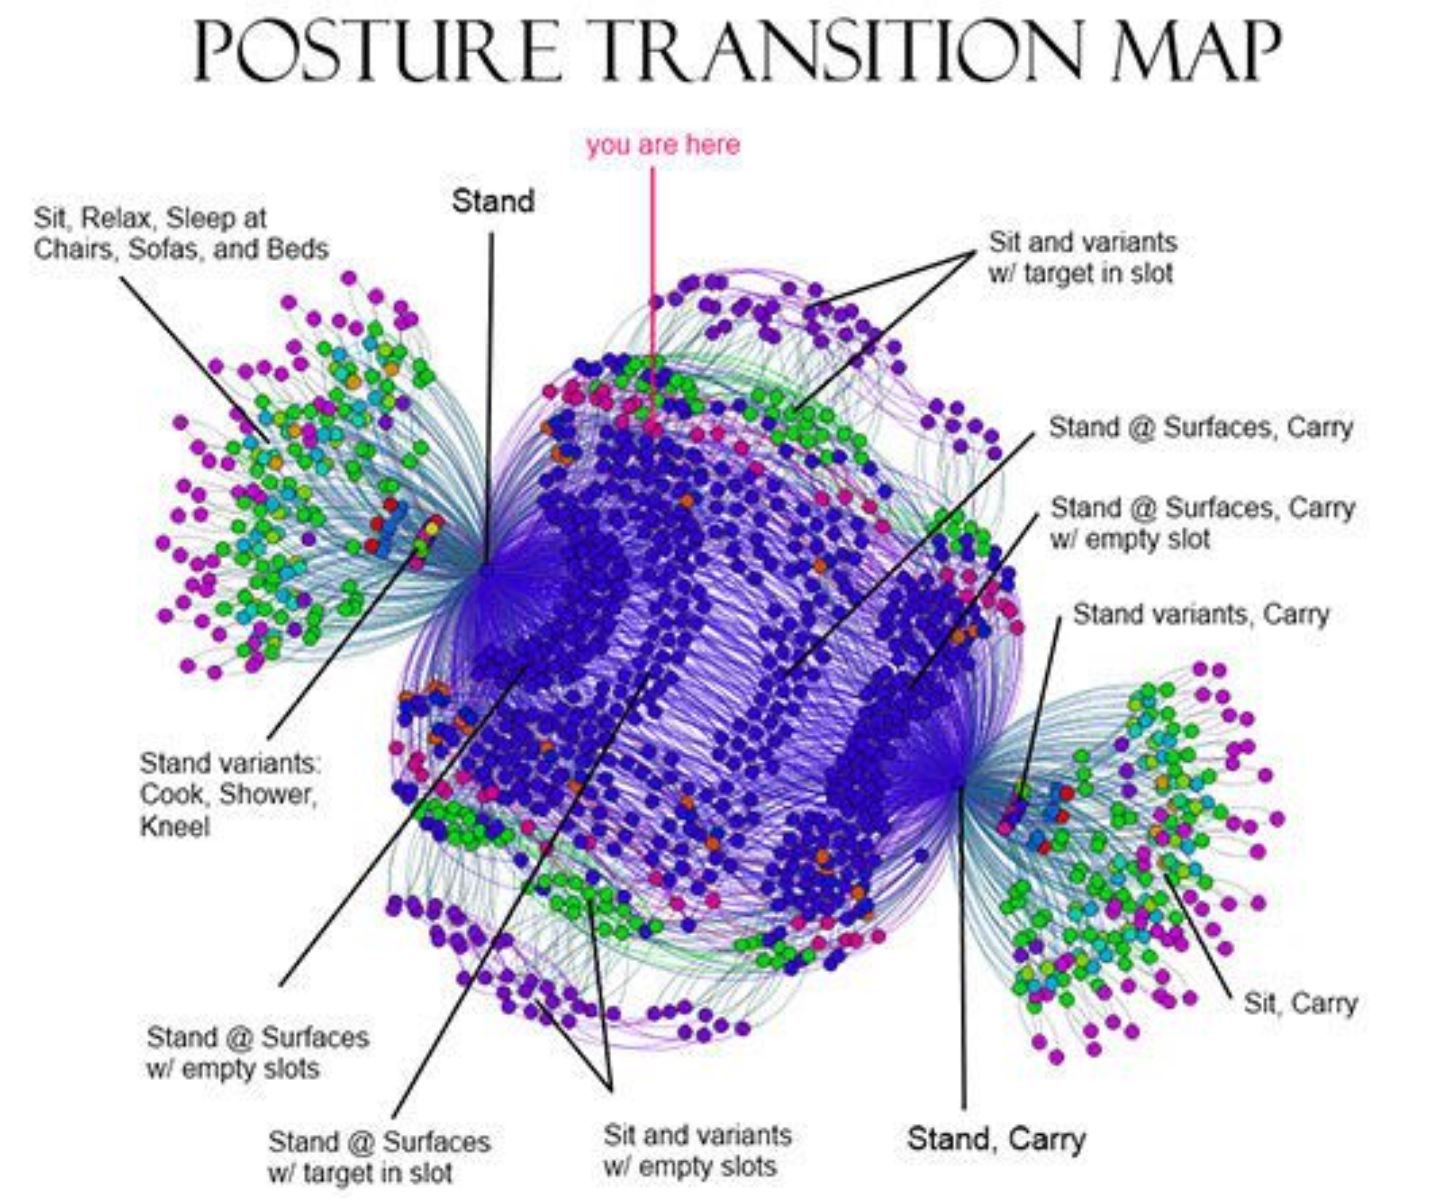
\includegraphics{Figures/sims.JPG}
\decoRule
\caption[Le potentiel des conséquences d'un changement de posture d'un Sim dans Les Sims 4]{Cette image visualise le potentiel des conséquences d'un changement de posture d'un Sim dans Les Sims 4}
\label{fig:sims}
\end{figure}


~\par
"Dans de nombreux autres jeux, l'IA est étrangère au joueur quant à la manière dont elle se comporte. L'IA commande aux personnages de faire des choses fondamentalement différentes de celles des joueurs ... Ils opèrent dans un monde différent avec des possibilités différentes", explique Ingebretson. “Dans Les Sims, si vous restez assis à regarder votre ordinateur pendant un moment, l'IA prendra le contrôle et contrôlera également les actions de vos sims. Cela signifie que notre IA  doit prendre des décisions plus crédibles afin que le cours de l’action reste cohérent “\parencite{simsArticle}.

~\par
Écouter Ingebretson qui décrit les tenants et les aboutissants de l’intelligence artificielle dans The Sims 4 ressemble à un cours de psychologie humaine. À la base, l'IA travaille avec l'interaction de deux mécanismes: les commodités et les courbes d'utilité. Les commodités représentent l'état interne d'un Sim, tandis qu'une courbe d'utilité dicte le désir d’un avatar à améliorer ses commodités. Chaque interaction ouvre une série d'améliorations possibles. "Par exemple, si un Sim boit une tasse de café, son énergie va monter mais sa vessie va baisser", dit Ingebretson. Comme dans le monde réel, tout est un compromis. Ainsi, lorsqu'il prend chaque décision, un Sim considère toutes les actions possibles, analyse leurs résultats, référence la courbe d'utilité et sélectionne la meilleure. Cependant, ces actions sont quelque peu aléatoires de par leur conception, de sorte que l'IA puisser donner l’illusion qu’elle est imprévisible.

~\par
Cet échange en une fraction de seconde entre la prise de contrôle de l’IA et du joueur est ce que Ingebretson appelle «autonomie», ou lorsqu'un sim est en pilote automatique. Dans les jeux précédents des Sims, l’autonomie était un système de départ et d’arrêt. Une fois qu'un sim a terminé avec une action, il s'exécute de manière autonome. Dans Les Sims 4, les développeurs ont amélioré l'efficacité de l'IA en créant une hiérarchie d'autonomie. "Au lieu de tout considérer dans le monde entier chaque fois qu'un Sim décide quoi faire, nous évaluons d'abord tous les produits de base et déterminons quels types d’actions sont les plus importantes pour le Sim", explique Ingebretson. "Cela nous permet d'éliminer de nombreuses possibilités." Cela signifie que les Sims deviennent plus rapides et plus efficaces pour prendre des décisions et peuvent effectuer plusieurs tâches plutôt que de suivre un script strict «d'abord ceci, ensuite cela» \parencite{simsArticle}.

~\par
Toutes ces améliorations et ces avancées rendent un jeu plus naturel, mais quand est-ce qu’un système d'intelligence artificielle devient-il trop efficace? "C'est un sujet intéressant que nous traitons dans chacun de ces projets, car nous pouvons continuer à rendre les Sims suffisamment intelligents pour mener leur propre vie", a déclaré Pearson. "Qu'est-ce qui est trop intelligent?"

~\par

Laissée à ses propres appareils parfaitement optimisés, l'IA pourrait facilement prendre le contrôle et jouer au jeu pour vous, laissant ainsi aux Sims effectuer un nombre anormal d'actions en même temps ou annuler l'interaction du joueur. L’équipe a introduit des seuils de retard et d’attention pour limiter artificiellement le système. "Il est impossible pour un cerveau humain de gérer autant de flux d'entrées", explique Ingebretson. "Pour les Sims, nous construisons un modèle de la vie humaine. Nous devons modéliser les fautes des gens ainsi que leur efficacité" \parencite{simsArticle}. 

~\par
Nous pouvons apercevoir que l'approche dans Les Sims 4 afin de rendre l’IA plus crédible est différente du cas précédent, même si les deux approches ont des similitudes dans la complexité de leur modèle, qui consiste à alimenter les personnages d’un grand nombre de conditions détaillées et en cascade ( un geste, une quantité d’alcool consommée, une intonation...), avec des scénarios différents pour chaque état, c’est tout ces détails qui donnent l’illusion de la réalité.

~\par
En plus de cela, Les Sims 4 propose un système tout à fait novateur, qui consiste en la prise de contrôle de l’IA du personnage joué par l’utilisateur lors des moments où celui-ci est au repos (quand le joueur laisse tourner le jeu sans y toucher). Mais celle-ci ne le fait pas n’importe comment, elle le fait tout en restant cohérente avec l’état précédent de l’agent, par exemple si le personnage est en train de boire de l’eau et que l’IA intervient et en prend le contrôle, elle le pousse à laver son verre, avant de l'essuyer de le ranger dans l’évier.

~\par
En plus de cela, les fautes des gens ainsi que leurs moments d'inattention et de faiblesse ont aussi été modélisés, non pas de manière directe, mais en introduisant des seuils de retards dans la succession des actions, afin que celles-ci aient l’air naturelles, et qu’elles ne ressemblent pas à un flot ininterrompu d’actions, comportement  qui n’est pas compréhensible par l’homme.
